\documentclass[tikz,border=12pt]{standalone}
\usepackage[T1]{fontenc}
\usepackage{mathpazo}
\usepackage{amsmath,amssymb}
\usetikzlibrary{arrows.meta}

\definecolor{stblue}{HTML}{7B97AD}
\definecolor{rwgold}{HTML}{B8995E}
\definecolor{sage}{HTML}{7A9A7E}
\definecolor{dkbrown}{HTML}{3D3530}
\definecolor{wmgray}{HTML}{7B7067}
\definecolor{cream}{HTML}{F9F6F0}
\definecolor{border}{HTML}{D4C9B8}
\definecolor{terracotta}{HTML}{C47A6A}
\definecolor{lavender}{HTML}{907EA0}

\begin{document}
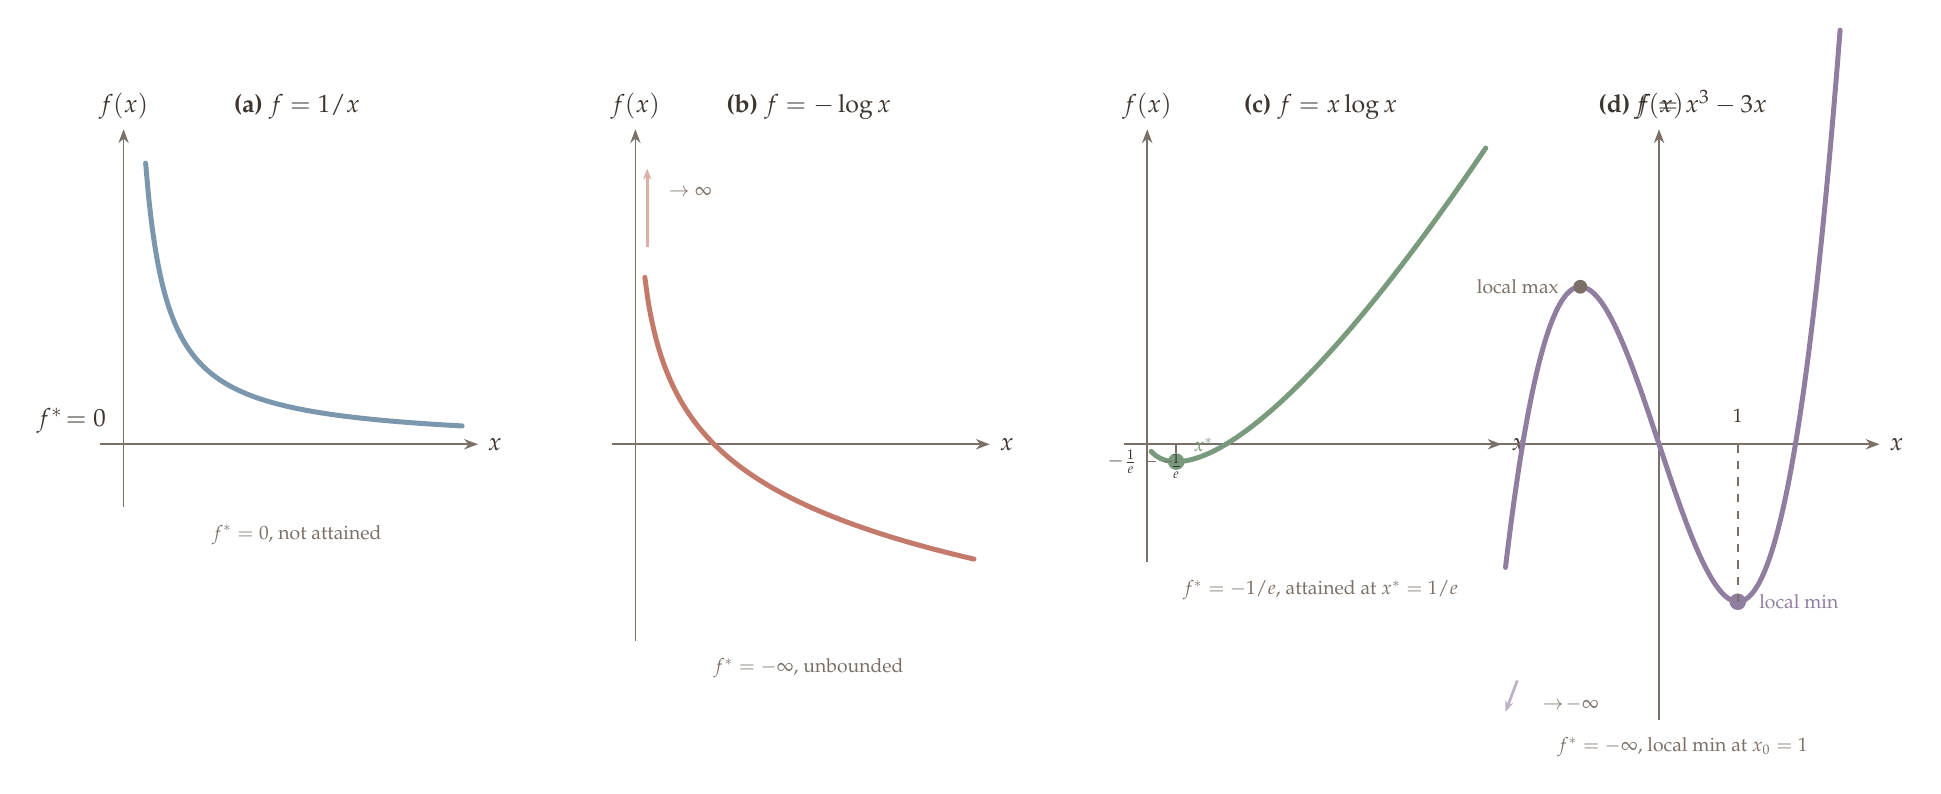
\begin{tikzpicture}[
  axis/.style={-{Stealth[length=5pt]}, wmgray, line width=0.6pt},
  curve/.style={line width=1.8pt, line cap=round},
  dashed line/.style={dashed, wmgray, line width=0.6pt},
  label/.style={dkbrown, font=\small},
]

% ===== Panel (a): f = 1/x on R++ =====
\begin{scope}[shift={(0,0)}]
  % axes
  \draw[axis] (-0.3,0) -- (4.5,0) node[right, label] {$x$};
  \draw[axis] (0,-0.8) -- (0,4) node[above, label] {$f(x)$};

  % f* = 0 dashed line
  \draw[dashed line] (-0.3,0) -- (4.3,0);
  \node[label, anchor=east] at (-0.1,0.3) {$f^*\!=0$};

  % curve: 1/x
  \draw[curve, stblue, domain=0.28:4.3, samples=100, smooth]
    plot (\x, {1/\x});

  % title
  \node[dkbrown, font=\small\bfseries, anchor=south] at (2.2,4) {(a) $f = 1/x$};
  \node[wmgray, font=\scriptsize, anchor=north] at (2.2,-0.9) {$f^*=0$, not attained};
\end{scope}

% ===== Panel (b): f = -log(x) on R++ =====
\begin{scope}[shift={(6.5,0)}]
  % axes
  \draw[axis] (-0.3,0) -- (4.5,0) node[right, label] {$x$};
  \draw[axis] (0,-2.5) -- (0,4) node[above, label] {$f(x)$};

  % curve: -ln(x), shifted so it looks nice
  \draw[curve, terracotta, domain=0.12:4.3, samples=100, smooth]
    plot (\x, {-ln(\x)});

  % arrow indicating unbounded below
  \draw[-{Stealth[length=4pt]}, terracotta!60, line width=1pt] (0.15,2.5) -- (0.15,3.5);
  \node[wmgray, font=\scriptsize, anchor=west] at (0.3,3.2) {$\to\infty$};

  % title
  \node[dkbrown, font=\small\bfseries, anchor=south] at (2.2,4) {(b) $f = -\log x$};
  \node[wmgray, font=\scriptsize, anchor=north] at (2.2,-2.6) {$f^*=-\infty$, unbounded};
\end{scope}

% ===== Panel (c): f = x log(x) on R++ =====
\begin{scope}[shift={(13,0)}]
  % axes
  \draw[axis] (-0.3,0) -- (4.5,0) node[right, label] {$x$};
  \draw[axis] (0,-1.5) -- (0,4) node[above, label] {$f(x)$};

  % scale: x in [0,4], plot x*ln(x) but we need to scale
  % x*ln(x): min at x=1/e ≈ 0.368, f(1/e) = -1/e ≈ -0.368
  % at x=4: 4*ln(4) ≈ 5.55 -- too big, let's scale y by 0.6
  \draw[curve, sage, domain=0.05:4.3, samples=150, smooth]
    plot (\x, {0.6*\x*ln(\x)});

  % mark minimum at x = 1/e
  \pgfmathsetmacro{\xmin}{1/exp(1)}
  \pgfmathsetmacro{\ymin}{0.6*\xmin*ln(\xmin)}
  \fill[sage] (\xmin, \ymin) circle (3pt);

  % dashed lines to minimum
  \draw[dashed line] (\xmin, 0) -- (\xmin, \ymin);
  \draw[dashed line] (0, \ymin) -- (\xmin, \ymin);
  \node[label, anchor=north, font=\scriptsize] at (\xmin, 0) {$\frac{1}{e}$};
  \node[label, anchor=east, font=\scriptsize] at (0, \ymin) {$-\frac{1}{e}$};

  % star at minimum
  \node[sage, font=\scriptsize, anchor=south west] at (\xmin+0.1, \ymin) {$x^*$};

  % title
  \node[dkbrown, font=\small\bfseries, anchor=south] at (2.2,4) {(c) $f = x\log x$};
  \node[wmgray, font=\scriptsize, anchor=north] at (2.2,-1.6) {$f^*=-1/e$, attained at $x^*=1/e$};
\end{scope}

% ===== Panel (d): f = x^3 - 3x on R =====
\begin{scope}[shift={(19.5,0)}]
  % axes
  \draw[axis] (-2.3,0) -- (2.8,0) node[right, label] {$x$};
  \draw[axis] (0,-3.5) -- (0,4) node[above, label] {$f(x)$};

  % curve: x^3 - 3x
  \draw[curve, lavender, domain=-1.95:2.3, samples=100, smooth]
    plot (\x, {\x*\x*\x - 3*\x});

  % mark local min at x=1, f(1)=-2
  \fill[lavender] (1,-2) circle (3pt);
  \draw[dashed line] (1,0) -- (1,-2);
  \node[label, anchor=south, font=\scriptsize] at (1,0.15) {$1$};
  \node[lavender, font=\scriptsize, anchor=west] at (1.15,-2) {local min};

  % mark local max at x=-1, f(-1)=2
  \fill[wmgray] (-1,2) circle (2.5pt);
  \node[wmgray, font=\scriptsize, anchor=east] at (-1.15,2) {local max};

  % arrow indicating f -> -infty
  \draw[-{Stealth[length=4pt]}, lavender!60, line width=1pt] (-1.8,-3) -- (-1.95,-3.4);
  \node[wmgray, font=\scriptsize, anchor=west] at (-1.6,-3.3) {$\to\!-\infty$};

  % title
  \node[dkbrown, font=\small\bfseries, anchor=south] at (0.3,4) {(d) $f = x^3-3x$};
  \node[wmgray, font=\scriptsize, anchor=north] at (0.3,-3.6) {$f^*=-\infty$, local min at $x_0=1$};
\end{scope}

\end{tikzpicture}
\end{document}
